\documentclass[a4paper]{article}
\usepackage[utf8]{inputenc}
\usepackage{amsmath}
\usepackage{amssymb}
\usepackage{caption}
\usepackage{mathtools}
\usepackage{amsfonts}
\usepackage{lastpage}
\usepackage{tikz}
\usepackage{float}
\usepackage{textcomp}
\usetikzlibrary{patterns}
\usepackage{pdfpages}
\usepackage{gauss}
\usepackage{fancyvrb}
\usepackage[table]{colortbl}
\usepackage{fancyhdr}
\usepackage{graphicx}
\usepackage[margin=2.5 cm]{geometry}

\definecolor{listinggray}{gray}{0.9}
\usepackage{listings}
\lstset{
	language=,
	literate=
		{æ}{{\ae}}1
		{ø}{{\o}}1
		{å}{{\aa}}1
		{Æ}{{\AE}}1
		{Ø}{{\O}}1
		{Å}{{\AA}}1,
	backgroundcolor=\color{listinggray},
	tabsize=3,
	rulecolor=,
	basicstyle=\scriptsize,
	upquote=true,
	aboveskip={0.2\baselineskip},
	columns=fixed,
	showstringspaces=false,
	extendedchars=true,
	breaklines=true,
	prebreak =\raisebox{0ex}[0ex][0ex]{\ensuremath{\hookleftarrow}},
	frame=single,
	showtabs=false,
	showspaces=false,
	showlines=true,
	showstringspaces=false,
	identifierstyle=\ttfamily,
	keywordstyle=\color[rgb]{0,0,1},
	commentstyle=\color[rgb]{0.133,0.545,0.133},
	stringstyle=\color[rgb]{0.627,0.126,0.941},
  moredelim=**[is][\color{blue}]{@}{@},
}

\lstdefinestyle{base}{
  emptylines=1,
  breaklines=true,
  basicstyle=\ttfamily\color{black},
}

\pagestyle{fancy}
\def\checkmark{\tikz\fill[scale=0.4](0,.35) -- (.25,0) -- (1,.7) -- (.25,.15) -- cycle;}
\newcommand*\circled[1]{\tikz[baseline=(char.base)]{
            \node[shape=circle,draw,inner sep=2pt] (char) {#1};}}
\newcommand*\squared[1]{%
  \tikz[baseline=(R.base)]\node[draw,rectangle,inner sep=0.5pt](R) {#1};\!}
\newcommand{\comment}[1]{%
  \text{\phantom{(#1)}} \tag{#1}}
\def\el{[\![}
\def\er{]\!]}
\def\dpip{|\!|}
\def\MeanN{\frac{1}{N}\sum^N_{n=1}}
\cfoot{Page \thepage\ of \pageref{LastPage}}
\DeclareGraphicsExtensions{.pdf,.png,.jpg}
\author{Nikolaj Dybdahl Rathcke (rfq695) \\ Victor Petren Bach Hansen (grn762)}
\title{Randomized Algorithms \\ Assignment 1}
\lhead{Randomized Algorithms}
\rhead{Assignment 1}

\begin{document}
\maketitle

\section*{Summary of chapter 1}
\subsection*{Min-cut algorithm}
An algorithm to find a min-cut in an undirected graph $G$ is to pick an edge and contract it. We keep doing this until only two vertices remain and the number of edges between should supposedly be a min-cut. It is not always true, but we can bound the probability it is incorrect. \\
\\
Let $C$ be a min-cut of size $k$. The graph has at least $kn/2$ edges. Thus the probability of picking an edge belonging to the min-cut $C$ is $k/(nk/2)=2/n$ or $1-2/n$ for not picking an edge belonging to the min-cut. When we pick the next edge, it has probability of $1-2/(n-1)$ for not belonging to $C$. Generally for all $n-2$ iteration, there is a probability of $1-2/(n-i+1)$ for not picking an edge belonging to $C$.\\
We write this probability as $P[\cap_{i=1}^{n-2} \xi_i]\geq \prod_i^{n-2} (1-\frac{2}{n-i+1})=\frac{2}{n(n-1)}$.\\

This is not very big, but we can run the algortihm many times (picking random edges each time) to minimize the probability that the algorithms fails. Good when no efficient algorithm exists.

We call an algorithm which sometimes produces an incorrect answer, whose probability we are able to bound, a Monte Carlo algorithm.

\subsection*{Binary planar partition}
We define the binary planar partition, of a set of size $n$ non-intersecting linesegments $S=\{s_1,s_2, \ldots, s_n\}$, as binary tree where each internal node $v$ in the tree is a region $r(v)$ of the plane. The root node of the tree corresponds to the entire plane. Each internal node is then intersected by the line $l(v)$ into two new regions. Given $S$ we then want to find a binary planar partition s.t. each region atmost contains one line segment $s_i$. Note that a line segment can be
split into multiple if intersected by a line $l(v)$ s.t. each part lies within a different region.\\


Within the field of computer graphics, we can use binary planar partitions to solve the problem of \textit{hidden line elimination}. For some given direction of viewing, we can use the idea of \texttt{painter's algorithm} which consists of drawing the objects that are furthest behind first and then progressively drawing objects that are nearer. With a BPP, we can recursively traverse the tree as follows. At the root, decide which side of the partition line $L_1$ is further away than the other
and the render the objects in that subtree recursively, after that render the other side recursively.

The time it takes to render everything then obviously depends on the size of the tree, which means we want it to be as small as possible. Since line segments can be split into multiple segments, we cannot be sure of a partition of size $\mathcal{O}(n)$.\\

The algorithm RandAuto describes a fast randomized approach to constructing a BPP of expected size $\mathcal{O}(n\log n)$. Consider a line segment $s$. Let $l(s)$ then be the line obtained by extending $s$ infinitely on both sides. From the set $S$, we can then construct an \textit{autopartition}, which is a BPP, by only using intersecting lines from the set $\{l(s_1), l(s_2),\ldots,l(s_n)\}$.

Given the set $S$, RandAuto then works by first picking a permutation $\pi$ of $\{1,2,\ldots,n\}$ uniformly at random. Then while any regions contains more than one line segment, we partition the plane with the line $l(s_i)$ where $i$ is the first in the ordering $\pi$ s.t. $s_i$ cuts that region.


\section*{Summary of chapter 2}
N/A
\section*{Exercise 1.2}
To prove there are inputs where the possibility of finding a min-cut is exponentially low, we just need to find some graph family $\mathbb{F}$ which has an exponentially low probability. \\
Consider the graphs which consist of two complete graphs of size $n$, $K_n$, which are connected by a single edge. For analysis sake, both complete graphs must have size $n$. Figure \ref{fig1} shows the graph type with $n=3$.
\begin{figure}[H]
  \centering
  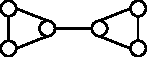
\includegraphics[scale=2]{fig1.pdf}
  \caption{Two complete graphs of size $n$ connected by a single edge}
  \label{fig1}
\end{figure}
Now we want to show that the probability of getting a correct result with this type of graph is exponentially small when we contract vertices instead of edges. We see that if contract two vertices that belong to different $K_n$, it will join the graphs in a one vertex. This means our optimal cut no longer has size $1$. To see that the probability of this \textit{not} happening in any of the $n-2$ iteration, call the event of successfully contracting each complete graph into a single vertex (that the remaining two nodes are the contractions of all the nodes from their original $K_n$) for $A$. We also know that for a result to be correct, each of the remaining nodes are the contraction of exactly $n$ nodes (not nessecarily a correct solution). Call this type of event for $B$. Now, the number of events of type $B$ are actually the number of ways we can pick $n$ nodes out of $2n$ nodes, namely $\binom{2n}{n}$. Of this number, only $2$ of them are events of type $A$. These are the cases where we pick the $n$ nodes from either the first or the second complete graph. So we have the probability of success (event $A$) is:
\begin{align*}
  \mathbb{P}\left[ A \right] &= \mathbb{P}\left[A|B\right]\left[B\right] \\
                             &\leq \frac{2}{\binom{2n}{n}} \comment{Bounding the probability by removing an event $B$} \\
                             &\leq\frac{2}{\left(\frac{2ne}{n}\right)^n} \comment{As $\binom{n}{k}\leq \left(\frac{ne}{k}\right)^k$.} \\
                             &=\frac{2}{\left(2e\right)^n}
\end{align*}
Which shows the probability is exponentially small in the number of vertices for the graph. Note we remove the probability of event $B$ happening in the first place. This is because by removing it, it only makes the probability greater - an upper bound. It also allows us to disregard the probability of event $B$ happening in the first place to avoid counting all possible outcomes.

\section*{Exercise 1.3}
To get an expected running time of $\frac{T(n)+t(n)}{\gamma (N)}$, we do the obvious. We run the Monte Carlo algorithm in $T(n)$ time and then validate it in $t(n)$ time. The fraction comes from getting the probability of getting the result right. We can expect that we need to run the Monte Carlo algorithm $1/\gamma (n)$ times and therefore we can expected the validation algorithm $1/\gamma (n)$ times. Multiplying the running times for two algorithm into the numerator yields the desired expected running time.

\section*{Problem 1.1}
\subsection*{(a)}
Let $T$ be tails and $H$ be heads. We devise a scheme that tosses the coin twice. If the coin has the same result, then we disregard the result and toss it twice again. If the results are different, we pick the first (or second, as long as it is chosen beforehand) result. The reason this generates unbiased coin-flips is that the probability of gettings $TH$ is the same as getting $HT$ since they are independent flips. The other two scenarios are disregarded, meaning the probability the choice comes from either of these events is $0$. Thus we have a $50$ percent probability on the remaining events. Note that $p>0$ or we will end up throwing the coin forever.\\
If the probability of getting $H$ is $p$, then the probability of $T$ is $1-p$. Now, the expected number of rounds  (throwing it twice) before getting a result must be $\frac{1}{2p(1-p)}$ - the probability that either $TH$ or $HT$ happens . If we want to count the number of throws of the coin, we simply multiply the result by $2$, yielding:
$$
\mathbb{E}\left[ \mbox{\# of throws} \right]=\frac{2}{2p(1-p)}=\frac{1}{p(1-p)}
$$
which is what we wanted to show.

\subsection*{(b)}
We can extend the scheme to more "levels". That is, if we toss $H$ two times (a pair) on what we will call level $0$, we can count this as a single $H$ on level $1$. The following pretty ASCII example shows this idea:
\begin{verbatim}
  Level 0: H H H T T T
            |       |
  Level 1:  H       T
\end{verbatim}
As you can see, adopting the strategy from (a), we get an independent coin flip from the $HT$ throw in the middle, but not for the other two pairs. But we can also extract one from level $1$, as the probability of throwing $HHHTTT$ is the same as throwing $TTHTHH$. However, we have to still consider them in pairs, so the we cannot extract another independent throw from level $1$ in the following example:
\begin{verbatim}
  Level 0: H H H H H T T T
            |   |       |
  Level 1:  H   H       T
\end{verbatim}
Since if the probability of getting $H$ is significantly larger, then we would almost always extract an $H$ whenever we got a $TT$ in level $0$. So the idea is to extend this to arbitrary many level, so in another (larger) example:
\begin{verbatim}
  Level 0: H H H H H T T T T T
            |   |       |   |
  Level 1:  H   H       T   T
              |           |
  Level 2:    H           T
\end{verbatim}
We can extract another throw on level $2$. The idea is to extract as many as possible on each level if they are in a pair and otherwise they go through to the next level. \\
We don't know if this is optimal, but it will extract more independent throws than the strategy proposed in (a).

\section*{Problem 1.4}
\subsection*{(a)}
So we have some input with $n$ elements. The shuffle knows as the Knuth-shuffle (introduced by Durstenfeld) can generate a random permutation by iteratively swapping elements from one with another random one. This algorithm is probably easier to explain with the following pseudo-code on an input array $a$ with $n$ elements.:
\begin{lstlisting}
for (int i = 0; i < n-1; i++) {
  j = rand(0, n-i); // 0 inclusive and n-1 exclusive
  swap a[i] and a[j];
\end{lstlisting}
This algorithm is quite powerful as it runs in $\mathcal{O}(n)$ time (swaps are done in constant time) and it does it in-place, so we don't waste bits on auxillary data structures. The number of random bits depends on our random choice. For any choice we need at most $\lceil \lg n \rceil$ bits to represent the index. Since we do this $n$ times, we need $\mathcal{O}(n\lg n)$ bits to perform the algorithm. \\
There are no lower bounds for this algorithms, which means we can actually say it runs $\Theta(n)$ time and use $\Theta(n\lg n)$ bits.

\subsection*{(b)}
Yes, the scheme is a random permutation when the elements $a_n$ are tied to the random variables $X_n$. To easily see this, we can pick a random element $a_i$, the random variable $X_i$ has a probability of $1/n$ of being on the $n$'th position in the sorted list. Since this works for an arbitrary element, it must work for the entire permutation as well. \\
The scheme, however, is not particularly efficient. The running time is quite obviously $\mathcal{O}(n\lg n)$ as we need to sort the random variables. However, it also quite inefficient in terms of bits as we need $\mathcal{n\lg n}$ bits for the sorting as well.

\subsection*{(c)}
N/A


\section*{Problem 1.8}
\subsection*{(a)}
Imagine a graph that has the source $s$ and sink $t$, but also $n$ vertices $v_1,v_2,..,v_n$. Now we connected $s$ to each $v_i$ by a single edge and we connect each $v_i$ to $t$ with $k$ edges. Figure \ref{fig2} shows an example of this graph with $n=3$ and $k=2$.
\begin{figure}[H]
  \centering
  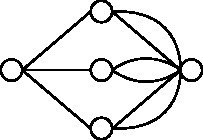
\includegraphics[scale=2]{fig2.pdf}
  \caption{The graph connected $s$ to $t$ through $3$ vertices and $k=2$.}
  \label{fig2}
\end{figure}
Now, for this type of graph, we would always have to contract an edge from $s$ to any other $v_i$. If we contract an edge between $v_i$ and $t$, it will increase the $s-t$ min-cut by $1$ (from $n$ to $n+1$ on the first iteration). Furthermore, every time we contract an edge between a vertex $v_i$ and $t$, we remove a total of $k+1$ edges as the edge from $s$ to $v_i$ will instead be connected to $t$ and therefore we cannot pick it in the next iteration. To have the algorithm give an optimal answer, we want to contract an edge from a vertex $v_i$ to $t$ in each iteration. We can write this probability as:
\begin{align*}
  \mathbb{P}\left[ \mbox{Optimal answer} \right] &= \prod_{i=0}^{n-1} \frac{kn-ki}{(k+1)n-(k+1)i} \\
                                                 &= \prod_{i=0}^{n-1} \frac{k(n-i)}{(k+1)(n-i)} \\
                                                 &= \prod_{i=0}^{n-1} \frac{k}{k+1} \\
                                                 &= \left( \frac{k}{k+1}\right) ^n
\end{align*}
Which shows the probability of getting an optimal answer is exponentially small in the number of vertices for this type of graph. Note that the actual number of vertices is $n+2$, but this still makes the probability exponentially small.

\subsection*{(b)}
If we consider the graph from (a) but where every $v_i$ is connected to $t$ by a single edge instead (see Figure \ref{fig3}), we see that to make an $s,t$ cut, we need to remove at least $n$ edges. If we remove ana incoming edge to a vertex $v_i$, we cannot pick the outcoming edge as it connect $s$ with $t$, and vice versa. This means we can pick only one of the two, and we need to make this choice $n$ times. This yields a total number of $2^n$ of $s,t$ min-cuts. We weren't able to produce a better result than this.
\begin{figure}[H]
  \centering
  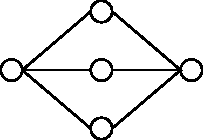
\includegraphics[scale=2]{fig3.pdf}
  \caption{The graph connected $s$ to $t$ through $3$ vertices and $k=1$.}
  \label{fig3}
\end{figure}

\end{document}
